% FPGA-Based Pulse Simulator Proposal for MeitY
% Submitted by CDAC Noida
% Document Class: Article

\documentclass[12pt,a4paper]{article}

% Required Packages
\usepackage{amsmath}
\usepackage{amssymb}
\usepackage{amsthm}
\usepackage{physics}
\usepackage{mathtools}
\usepackage{bm}
\usepackage{tikz}
\usepackage{pgfplots}
\usepackage[margin=1in]{geometry}
\usepackage{hyperref}
\usepackage{cleveref}
\usepackage{graphicx}
\usepackage[backend=biber,style=numeric,sorting=nyt]{biblatex}
\usepackage{booktabs}
\usepackage{array}
\usepackage{longtable}
\usepackage{xcolor}
\usepackage{enumitem}
\usepackage{fancyhdr}

% TikZ Libraries
\usetikzlibrary{shapes.geometric, arrows.meta, positioning, calc, decorations.pathreplacing, fit, backgrounds}
\pgfplotsset{compat=1.18}

% Hyperref Setup
\hypersetup{
    colorlinks=true,
    linkcolor=blue,
    filecolor=magenta,
    urlcolor=cyan,
    citecolor=green!50!black,
    pdftitle={FPGA-Based Pulse Simulator for Quantum and Classical Signal Research},
    pdfauthor={CDAC Noida},
}

% Custom Commands
\newcommand{\rupees}[1]{\text{₹}#1}
\newcommand{\crore}[1]{\rupees{#1}\text{ crores}}
\newcommand{\hamiltonian}{\mathcal{H}}
\newcommand{\pauli}[1]{\sigma_{#1}}

% Theorem Environments
\theoremstyle{definition}
\newtheorem{definition}{Definition}[section]
\newtheorem{objective}{Objective}[section]

% Header/Footer
\pagestyle{fancy}
\fancyhf{}
\rhead{CDAC Noida}
\lhead{FPGA-Based Pulse Simulator Proposal}
\rfoot{Page \thepage}

% Bibliography File (inline)
\usepackage{filecontents}
\begin{filecontents}{references.bib}
@book{nielsen2010quantum,
  author    = {Nielsen, Michael A. and Chuang, Isaac L.},
  title     = {Quantum Computation and Quantum Information},
  publisher = {Cambridge University Press},
  year      = {2010},
  edition   = {10th Anniversary},
  isbn      = {978-1107002173}
}

@article{krantz2019quantum,
  author  = {Krantz, Philip and Kjaergaard, Morten and Yan, Fei and Orlando, Terry P. and Gustavsson, Simon and Oliver, William D.},
  title   = {A Quantum Engineer's Guide to Superconducting Qubits},
  journal = {Applied Physics Reviews},
  volume  = {6},
  number  = {2},
  pages   = {021318},
  year    = {2019},
  doi     = {10.1063/1.5089550}
}

@article{motzoi2009simple,
  author  = {Motzoi, F. and Gambetta, J. M. and Rebentrost, P. and Wilhelm, F. K.},
  title   = {Simple Pulses for Elimination of Leakage in Weakly Nonlinear Qubits},
  journal = {Physical Review Letters},
  volume  = {103},
  number  = {11},
  pages   = {110501},
  year    = {2009},
  doi     = {10.1103/PhysRevLett.103.110501}
}

@inproceedings{fu2017fpga,
  author    = {Fu, X. and Riesebos, L. and Lao, L. and Almudever, C. G. and Sebastiano, F. and Versluis, R. and Charbon, E. and Bertels, K.},
  title     = {A Microarchitecture for a Superconducting Quantum Processor},
  booktitle = {IEEE/ACM International Symposium on Microarchitecture (MICRO)},
  pages     = {813--825},
  year      = {2017},
  doi       = {10.1145/3123939.3123952}
}

@article{rol2020time,
  author  = {Rol, M. A. and Battistel, F. and Malinowski, F. K. and Bultink, C. C. and Tarasinski, B. M. and Vollmer, R. and Haider, N. and Langford, N. K. and DiCarlo, L.},
  title   = {Time-Domain Characterization and Correction of On-Chip Distortion of Control Pulses in a Quantum Processor},
  journal = {Applied Physics Letters},
  volume  = {116},
  number  = {5},
  pages   = {054001},
  year    = {2020},
  doi     = {10.1063/1.5133894}
}

@book{kaye2007introduction,
  author    = {Kaye, Phillip and Laflamme, Raymond and Mosca, Michele},
  title     = {An Introduction to Quantum Computing},
  publisher = {Oxford University Press},
  year      = {2007},
  isbn      = {978-0198570493}
}

@article{werninghaus2021leakage,
  author  = {Werninghaus, M. and Egger, D. J. and Roy, F. and Machnes, S. and Wilhelm, F. K. and Filipp, S.},
  title   = {Leakage Reduction in Fast Superconducting Qubit Gates via Optimal Control},
  journal = {npj Quantum Information},
  volume  = {7},
  number  = {1},
  pages   = {14},
  year    = {2021},
  doi     = {10.1038/s41534-020-00346-2}
}

@article{penrose2010cycles,
  author  = {Penrose, Roger},
  title   = {Cycles of Time: An Extraordinary New View of the Universe},
  journal = {The Bodley Head},
  year    = {2010},
  note    = {Conformal Cyclic Cosmology (CCC) provides philosophical context for cyclic computational paradigms}
}

@article{sank2016fast,
  author  = {Sank, Daniel and Chen, Zijun and Khezri, Mostafa and Kelly, Julian and Barends, Rami and Campbell, Brooks and others},
  title   = {Measurement-Induced State Transitions in a Superconducting Qubit: Beyond the Rotating Wave Approximation},
  journal = {Physical Review Letters},
  volume  = {117},
  number  = {19},
  pages   = {190503},
  year    = {2016},
  doi     = {10.1103/PhysRevLett.117.190503}
}

@misc{xilinx2023ultrascale,
  author       = {{Xilinx Inc.}},
  title        = {UltraScale+ FPGA Product Tables and Product Selection Guide},
  year         = {2023},
  howpublished = {\url{https://www.xilinx.com/products/silicon-devices/fpga.html}},
  note         = {Accessed: 2024}
}
\end{filecontents}

\addbibresource{references.bib}

% Document Begin
\begin{document}

%=============================================================================
% TITLE PAGE
%=============================================================================
\begin{titlepage}
    \centering
    \vspace*{1cm}
    
    {\Large\bfseries Ministry of Electronics and Information Technology (MeitY)\\[0.3cm]
    Government of India}
    
    \vspace{1.5cm}
    
    {\Huge\bfseries Project Proposal}
    
    \vspace{1cm}
    
    \rule{\textwidth}{1.5pt}
    
    \vspace{0.5cm}
    
    {\LARGE\bfseries FPGA-Based Pulse Simulator for\\[0.3cm]
    Quantum and Classical Signal Research}
    
    \vspace{0.5cm}
    
    \rule{\textwidth}{1.5pt}
    
    \vspace{2cm}
    
    {\Large\textbf{Submitted by:}\\[0.3cm]
    Centre for Development of Advanced Computing (CDAC)\\
    Noida, Uttar Pradesh}
    
    \vspace{1.5cm}
    
    {\large\textbf{Project Duration:} 5 Years (60 Months)\\[0.3cm]
    \textbf{Total Budget:} \crore{5.0}\\[0.3cm]
    \textbf{Submission Date:} December 2024}
    
    \vfill
    
    \includegraphics[width=0.15\textwidth]{example-image}% Placeholder for CDAC logo
    
    \vspace{0.5cm}
    
    {\small Document Version 1.0 | Confidential}
    
\end{titlepage}

%=============================================================================
% ABSTRACT
%=============================================================================
\begin{abstract}
\noindent
This proposal presents a comprehensive five-year project to develop an indigenous \textbf{FPGA-Based Pulse Simulator} for quantum and classical signal research. The simulator will enable precise generation and manipulation of control pulses essential for quantum computing experiments, quantum algorithm validation, and advanced signal processing research.

The project leverages Field-Programmable Gate Arrays (FPGAs) to create a reconfigurable, high-fidelity pulse generation platform capable of simulating qubit control sequences, implementing arbitrary Hamiltonians, and interfacing with both simulated and physical quantum systems. The total project budget is \crore{5.0}, distributed across hardware procurement (\crore{2.0}), manpower (\crore{1.5}), software tools (\crore{0.5}), training and dissemination (\crore{0.5}), and contingency (\crore{0.5}).

Key deliverables include: (1) a fully functional FPGA-based pulse generation system with sub-nanosecond timing resolution, (2) comprehensive pulse libraries for standard quantum gates, (3) integration frameworks for quantum circuit simulators, (4) training modules for engineers and researchers, and (5) open-source release of core components to foster India's quantum computing ecosystem.

This initiative directly supports India's National Quantum Mission by establishing indigenous capabilities in quantum control hardware, reducing dependence on foreign technologies, and creating a skilled workforce in this strategically important domain.

\vspace{0.5cm}
\noindent\textbf{Keywords:} FPGA, Pulse Simulator, Quantum Computing, Qubit Control, Digital Signal Processing, Indigenous Development
\end{abstract}

\newpage
\tableofcontents
\newpage

%=============================================================================
% SECTION 1: EXECUTIVE SUMMARY
%=============================================================================
\section{Executive Summary}
\label{sec:executive_summary}

\subsection{Project Vision}

The \textbf{FPGA-Based Pulse Simulator} project aims to establish India as a self-reliant nation in quantum control hardware infrastructure. By developing an indigenous platform for generating, shaping, and analyzing quantum control pulses, this project addresses a critical gap in India's quantum technology ecosystem.

\subsection{Why MeitY Should Fund This Project}

\begin{enumerate}[label=\textbf{\arabic*.}, leftmargin=2cm]
    \item \textbf{National Capability in Quantum Simulation:} This project creates foundational infrastructure for quantum algorithm development and testing without requiring access to expensive quantum hardware. Researchers across India can validate quantum protocols using this simulator.
    
    \item \textbf{Indigenous FPGA Hardware Development:} The project strengthens CDAC's expertise in FPGA-based systems, contributing to India's semiconductor and electronics manufacturing ecosystem aligned with the ``Make in India'' initiative.
    
    \item \textbf{Training Ecosystem:} The project will train over 100 engineers and researchers in quantum control techniques, FPGA programming, and pulse-level quantum computing---skills essential for India's quantum workforce.
    
    \item \textbf{Strategic Autonomy:} By reducing dependence on imported quantum control systems, India gains strategic independence in a domain critical for national security and economic competitiveness.
    
    \item \textbf{Cost-Effective Solution:} At \crore{5.0} over five years, this project offers exceptional value compared to procuring commercial quantum control systems from abroad, which can cost several times more.
\end{enumerate}

\subsection{Expected Outcomes}

\begin{itemize}
    \item Fully functional FPGA-based pulse generation system with $<1$~ns timing jitter
    \item Pulse libraries implementing 50+ quantum gates
    \item Integration with Qiskit, Cirq, and other quantum frameworks
    \item 5 peer-reviewed publications in international journals
    \item Open-source release benefiting the global quantum community
    \item Trained workforce of 100+ quantum engineers
\end{itemize}

%=============================================================================
% SECTION 2: LAYMAN'S JUSTIFICATION
%=============================================================================
\section{Layman's Justification: Why This Project Matters}
\label{sec:layman}

\subsection{What Are We Building?}

\begin{quote}
\textit{``This project builds a machine that can mimic quantum pulses on reconfigurable chips (FPGAs). It helps India test quantum algorithms without needing expensive quantum computers.''}
\end{quote}

Imagine you want to learn how to fly an airplane. Before sitting in an actual cockpit, pilots train extensively on \textbf{flight simulators}---sophisticated machines that recreate the experience of flying without the risks and costs of real aircraft. Our project does the same thing, but for \textbf{quantum engineers}.

\subsection{The Flight Simulator Analogy}

\begin{center}
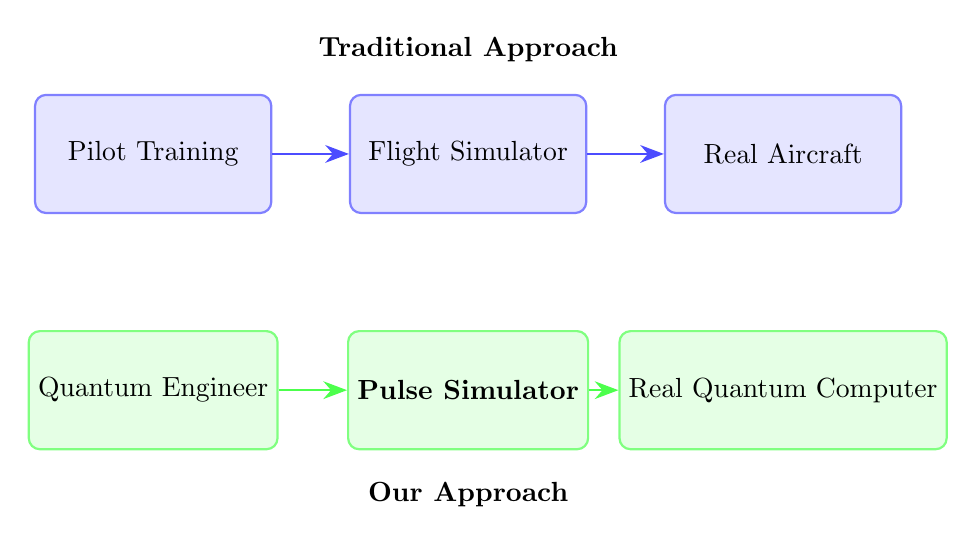
\begin{tikzpicture}[
    box/.style={rectangle, draw=blue!50, fill=blue!10, thick, minimum width=3cm, minimum height=1.5cm, text centered, rounded corners},
    arrow/.style={-{Stealth[length=3mm]}, thick, blue!70}
]
    % Flight Simulator
    \node[box] (pilot) at (0,0) {Pilot Training};
    \node[box] (flightsim) at (4,0) {Flight Simulator};
    \node[box] (realplane) at (8,0) {Real Aircraft};
    
    \draw[arrow] (pilot) -- (flightsim);
    \draw[arrow] (flightsim) -- (realplane);
    
    % Quantum Simulator
    \node[box, fill=green!10, draw=green!50] (qengineer) at (0,-3) {Quantum Engineer};
    \node[box, fill=green!10, draw=green!50] (pulsesim) at (4,-3) {\textbf{Pulse Simulator}};
    \node[box, fill=green!10, draw=green!50] (realquantum) at (8,-3) {Real Quantum Computer};
    
    \draw[arrow, green!70] (qengineer) -- (pulsesim);
    \draw[arrow, green!70] (pulsesim) -- (realquantum);
    
    % Labels
    \node[above=0.3cm] at (4,0.75) {\textbf{Traditional Approach}};
    \node[below=0.3cm] at (4,-3.75) {\textbf{Our Approach}};
\end{tikzpicture}
\end{center}

\textbf{Like a flight simulator for pilots, this is a pulse simulator for quantum engineers.}

\subsection{Why Is This Important for India?}

\subsubsection{Indigenous Hardware Development}
India currently imports most advanced quantum control equipment from countries like the USA, Europe, and China. This creates:
\begin{itemize}
    \item \textbf{Supply chain vulnerabilities}---geopolitical tensions can disrupt access
    \item \textbf{High costs}---imported systems cost \crore{10-50} or more
    \item \textbf{Technology dependence}---limited ability to customize for Indian needs
\end{itemize}

Our pulse simulator, built entirely in India using FPGAs, breaks this cycle.

\subsubsection{Skill Development}
The project will train engineers in:
\begin{itemize}
    \item FPGA design and programming
    \item Quantum computing fundamentals
    \item High-speed digital signal processing
    \item Hardware-software co-design
\end{itemize}

These skills are in high demand globally, and our trained workforce will contribute to India's technology leadership.

\subsubsection{Strategic Autonomy}
Quantum computing is expected to revolutionize:
\begin{itemize}
    \item Cryptography and cybersecurity
    \item Drug discovery and materials science
    \item Artificial intelligence and optimization
    \item Defense and national security applications
\end{itemize}

Having indigenous quantum control capabilities ensures India can pursue these applications independently.

\subsection{Simple Explanation of the Technology}

Quantum computers process information using \textbf{qubits}---the quantum equivalent of classical bits. Unlike regular bits (which are either 0 or 1), qubits can be in \textbf{superpositions}---existing as both 0 and 1 simultaneously.

To control qubits, we send them precisely shaped electrical \textbf{pulses}. These pulses must be:
\begin{itemize}
    \item \textbf{Extremely precise}---timing errors of billionths of a second matter
    \item \textbf{Perfectly shaped}---the pulse shape determines the quantum operation
    \item \textbf{Synchronized}---multiple qubits must receive coordinated pulses
\end{itemize}

Our FPGA-based simulator generates these pulses digitally, allowing researchers to:
\begin{enumerate}
    \item Design and test new quantum algorithms
    \item Validate pulse sequences before expensive experiments
    \item Train students on quantum control techniques
    \item Develop optimized pulse shapes for better quantum operations
\end{enumerate}

%=============================================================================
% SECTION 3: TECHNICAL FRAMEWORK
%=============================================================================
\section{Technical Framework}
\label{sec:technical}

\subsection{Quantum Control Theory Foundations}

\subsubsection{Qubit Hamiltonians}

The dynamics of a single qubit under external control are governed by the time-dependent Hamiltonian:

\begin{equation}
\boxed{
H(t) = \frac{\hbar \omega_0}{2}\sigma_z + \hbar \Omega(t)\sigma_x + \hbar \Delta(t)\sigma_y
}
\label{eq:hamiltonian}
\end{equation}

where:
\begin{itemize}
    \item $\hbar$ is the reduced Planck constant
    \item $\omega_0$ is the qubit transition frequency
    \item $\Omega(t)$ is the time-dependent control pulse amplitude (in-phase component)
    \item $\Delta(t)$ is the quadrature control pulse amplitude
    \item $\sigma_x, \sigma_y, \sigma_z$ are the Pauli matrices:
\end{itemize}

\begin{equation}
\sigma_x = \begin{pmatrix} 0 & 1 \\ 1 & 0 \end{pmatrix}, \quad
\sigma_y = \begin{pmatrix} 0 & -i \\ i & 0 \end{pmatrix}, \quad
\sigma_z = \begin{pmatrix} 1 & 0 \\ 0 & -1 \end{pmatrix}
\label{eq:pauli}
\end{equation}

For resonant driving (when the control pulse frequency matches $\omega_0$), the effective Hamiltonian in the rotating frame simplifies to:

\begin{equation}
H_{\text{eff}}(t) = \hbar \Omega(t)\sigma_x
\label{eq:hamiltonian_rotating}
\end{equation}

\subsubsection{Pulse Shaping Equations}

The control pulse $\Omega(t)$ can take various functional forms depending on the desired gate operation. The most common pulse shapes include:

\paragraph{Gaussian Pulse:}
\begin{equation}
\boxed{
\Omega(t) = \Omega_0 \exp\left(-\frac{(t-t_0)^2}{2\sigma^2}\right)
}
\label{eq:gaussian}
\end{equation}

where $\Omega_0$ is the peak amplitude, $t_0$ is the pulse center, and $\sigma$ is the pulse width parameter.

\paragraph{DRAG (Derivative Removal by Adiabatic Gate) Pulse:}
\begin{equation}
\Omega_{\text{DRAG}}(t) = \Omega_0 \exp\left(-\frac{(t-t_0)^2}{2\sigma^2}\right) \left[1 - \frac{\lambda}{\alpha} \cdot \frac{(t-t_0)}{\sigma^2}\right]
\label{eq:drag}
\end{equation}

where $\lambda$ is the DRAG coefficient and $\alpha$ is the qubit anharmonicity \cite{motzoi2009simple}.

\paragraph{Flat-Top Gaussian:}
\begin{equation}
\Omega_{\text{FT}}(t) = 
\begin{cases}
\Omega_0 \exp\left(-\frac{(t-t_r)^2}{2\sigma_r^2}\right) & t < t_r \\
\Omega_0 & t_r \leq t \leq t_f \\
\Omega_0 \exp\left(-\frac{(t-t_f)^2}{2\sigma_f^2}\right) & t > t_f
\end{cases}
\label{eq:flattop}
\end{equation}

\subsubsection{FPGA Digital Representation}

For FPGA implementation, continuous pulses must be discretized. Given a sampling period $\Delta t$, the discrete pulse samples are:

\begin{equation}
\boxed{
\Omega[n] = \Omega_0 \exp\left(-\frac{(n\Delta t - t_0)^2}{2\sigma^2}\right), \quad n = 0, 1, 2, \ldots, N-1
}
\label{eq:discrete}
\end{equation}

where $N$ is the total number of samples determining the pulse duration $T = N\Delta t$.

The digitized pulse is represented in fixed-point arithmetic with $B$ bits:
\begin{equation}
\Omega_{\text{digital}}[n] = \text{round}\left(\frac{\Omega[n]}{\Omega_{\text{max}}} \cdot (2^{B-1} - 1)\right)
\label{eq:digital}
\end{equation}

\begin{figure}[htbp]
\centering
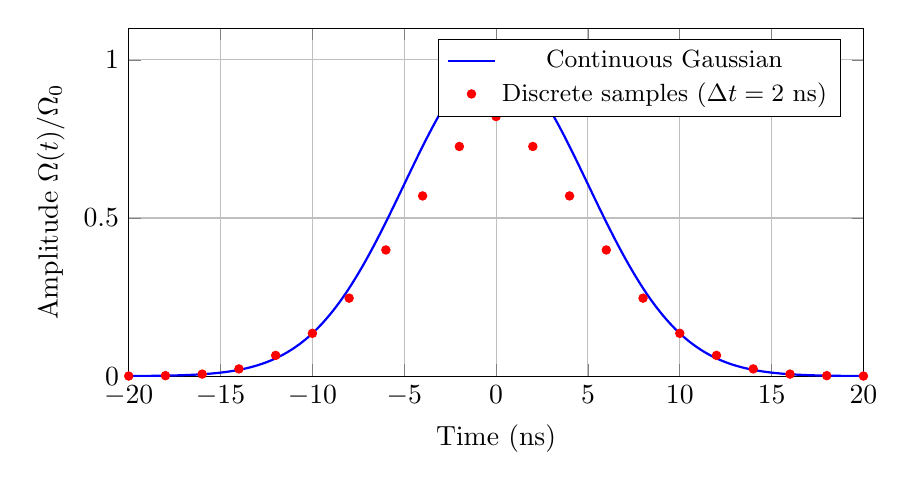
\begin{tikzpicture}
\begin{axis}[
    width=0.9\textwidth,
    height=6cm,
    xlabel={Time (ns)},
    ylabel={Amplitude $\Omega(t)/\Omega_0$},
    xmin=-20, xmax=20,
    ymin=0, ymax=1.1,
    grid=major,
    legend pos=north east,
    legend style={font=\small},
]
% Continuous Gaussian
\addplot[blue, thick, smooth, samples=100, domain=-20:20] 
    {exp(-x^2/(2*5^2))};
\addlegendentry{Continuous Gaussian}

% Discrete samples
\addplot[red, only marks, mark=*, mark size=1.5pt] 
    coordinates {
    (-20,0.0003) (-18,0.0015) (-16,0.0065) (-14,0.0228) (-12,0.0656)
    (-10,0.1353) (-8,0.2466) (-6,0.3989) (-4,0.5698) (-2,0.7261)
    (0,0.8208) (2,0.7261) (4,0.5698) (6,0.3989) (8,0.2466)
    (10,0.1353) (12,0.0656) (14,0.0228) (16,0.0065) (18,0.0015) (20,0.0003)
    };
\addlegendentry{Discrete samples ($\Delta t = 2$~ns)}

\end{axis}
\end{tikzpicture}
\caption{Continuous Gaussian pulse and its discrete FPGA representation. The FPGA generates samples at fixed time intervals $\Delta t$, which are then converted to analog signals via DAC.}
\label{fig:discretization}
\end{figure}

\subsubsection{Quantum Circuit Execution}

The time evolution operator for a qubit under control pulse $\Omega(t)$ is given by:

\begin{equation}
\boxed{
U(t) = \mathcal{T}\exp\left(-\frac{i}{\hbar}\int_0^t H(t') \, dt'\right)
}
\label{eq:evolution}
\end{equation}

where $\mathcal{T}$ denotes time-ordering. For simple cases, this reduces to:

\begin{equation}
U(\theta, \phi) = \exp\left(-i\frac{\theta}{2}(\cos\phi \, \sigma_x + \sin\phi \, \sigma_y)\right)
\label{eq:rotation}
\end{equation}

where the rotation angle $\theta$ is determined by the pulse area:
\begin{equation}
\theta = \int_0^T \Omega(t) \, dt
\label{eq:pulse_area}
\end{equation}

\subsection{Standard Quantum Gates via Pulse Sequences}

\subsubsection{Single-Qubit Gates}

\paragraph{Hadamard Gate (H):}
The Hadamard gate creates superposition and is implemented as:
\begin{equation}
H = \frac{1}{\sqrt{2}}\begin{pmatrix} 1 & 1 \\ 1 & -1 \end{pmatrix} = R_y\left(\frac{\pi}{2}\right) \cdot R_z(\pi)
\label{eq:hadamard}
\end{equation}

This requires a $\pi/2$ rotation about the $y$-axis followed by a $\pi$ rotation about the $z$-axis (implemented via phase shift).

\paragraph{Pauli-X Gate (NOT Gate):}
\begin{equation}
X = \sigma_x = \begin{pmatrix} 0 & 1 \\ 1 & 0 \end{pmatrix}
\label{eq:pauli_x}
\end{equation}

Implemented via a $\pi$-pulse: $\theta = \pi$, requiring:
\begin{equation}
\int_0^T \Omega(t) \, dt = \pi
\label{eq:pi_pulse}
\end{equation}

\paragraph{$R_x(\theta)$ and $R_y(\theta)$ Rotations:}
\begin{align}
R_x(\theta) &= \exp\left(-i\frac{\theta}{2}\sigma_x\right) = \cos\frac{\theta}{2}I - i\sin\frac{\theta}{2}\sigma_x \label{eq:rx}\\
R_y(\theta) &= \exp\left(-i\frac{\theta}{2}\sigma_y\right) = \cos\frac{\theta}{2}I - i\sin\frac{\theta}{2}\sigma_y \label{eq:ry}
\end{align}

\subsubsection{Two-Qubit Gates}

\paragraph{CNOT Gate:}
The controlled-NOT gate is the fundamental two-qubit entangling gate:
\begin{equation}
\text{CNOT} = \begin{pmatrix} 
1 & 0 & 0 & 0 \\
0 & 1 & 0 & 0 \\
0 & 0 & 0 & 1 \\
0 & 0 & 1 & 0
\end{pmatrix}
\label{eq:cnot}
\end{equation}

For superconducting qubits, CNOT is typically decomposed into:
\begin{equation}
\text{CNOT} = (I \otimes H) \cdot \text{CZ} \cdot (I \otimes H)
\label{eq:cnot_decomp}
\end{equation}

where CZ (controlled-Z) is implemented via cross-resonance pulses:
\begin{equation}
H_{\text{CR}}(t) = \Omega_{\text{CR}}(t) \left(\sigma_x^{(1)} \otimes I^{(2)} + \zeta \, \sigma_z^{(1)} \otimes \sigma_x^{(2)}\right)
\label{eq:cr_hamiltonian}
\end{equation}

\subsection{FPGA System Architecture}

The pulse simulator architecture consists of four main subsystems:

\begin{enumerate}
    \item \textbf{Digital Pulse Generator:} Synthesizes pulse waveforms from stored parameters
    \item \textbf{Digital-to-Analog Converter (DAC):} Converts digital samples to analog voltages
    \item \textbf{Analog Front-End:} Filters, amplifies, and conditions the output signals
    \item \textbf{Qubit Simulator Interface:} Connects to simulated or physical qubit systems
\end{enumerate}

\begin{figure}[htbp]
\centering
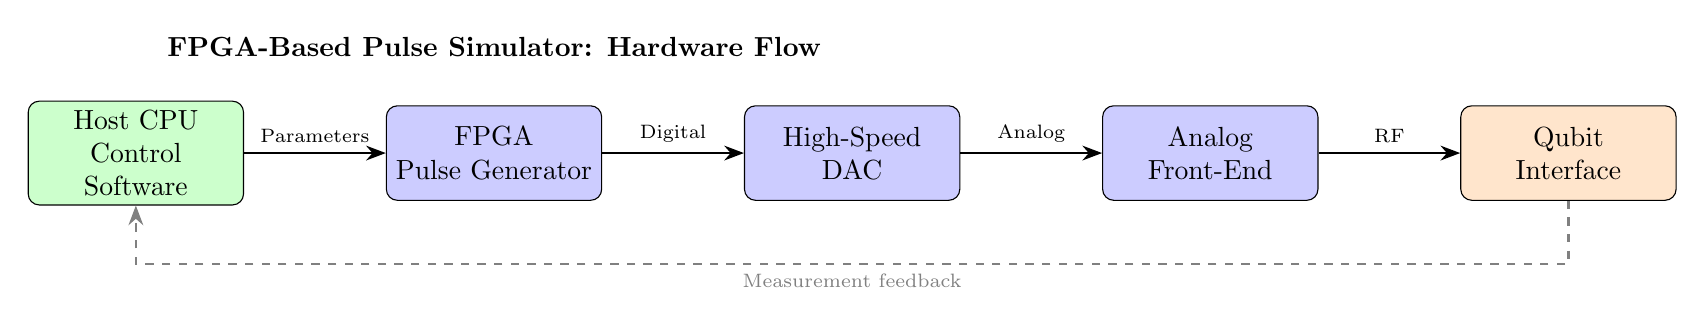
\begin{tikzpicture}[
    block/.style={rectangle, draw, fill=blue!20, text width=2.5cm, text centered, minimum height=1.2cm, rounded corners},
    arrow/.style={-{Stealth[length=2.5mm]}, thick},
    node distance=1.8cm
]
    % Main blocks
    \node[block, fill=green!20] (cpu) {Host CPU\\Control Software};
    \node[block, right=of cpu] (fpga) {FPGA\\Pulse Generator};
    \node[block, right=of fpga] (dac) {High-Speed\\DAC};
    \node[block, right=of dac] (afe) {Analog\\Front-End};
    \node[block, right=of afe, fill=orange!20] (qubit) {Qubit\\Interface};
    
    % Arrows
    \draw[arrow] (cpu) -- node[above, font=\scriptsize] {Parameters} (fpga);
    \draw[arrow] (fpga) -- node[above, font=\scriptsize] {Digital} (dac);
    \draw[arrow] (dac) -- node[above, font=\scriptsize] {Analog} (afe);
    \draw[arrow] (afe) -- node[above, font=\scriptsize] {RF} (qubit);
    
    % Feedback
    \draw[arrow, dashed, gray] (qubit.south) -- ++(0,-0.8) -| node[below, pos=0.25, font=\scriptsize] {Measurement feedback} (cpu.south);
    
    % Labels
    \node[above=0.5cm of fpga, font=\bfseries] {FPGA-Based Pulse Simulator: Hardware Flow};
    
\end{tikzpicture}
\caption{Block diagram of the FPGA-based pulse simulator hardware architecture.}
\label{fig:hardware_arch}
\end{figure}

\subsubsection{Specifications}

\begin{table}[htbp]
\centering
\caption{Target specifications for the FPGA-based pulse simulator}
\label{tab:specifications}
\begin{tabular}{@{}lll@{}}
\toprule
\textbf{Parameter} & \textbf{Target Value} & \textbf{Notes} \\
\midrule
Sampling Rate & 1--2 GSPS & Giga-samples per second \\
Timing Resolution & $<1$ ns & Sub-nanosecond jitter \\
Amplitude Resolution & 14--16 bits & DAC resolution \\
Number of Channels & 8--16 & Independent pulse channels \\
Pulse Memory & 1 GB & Per channel waveform storage \\
Maximum Pulse Duration & 10 $\mu$s & Configurable \\
Trigger Latency & $<50$ ns & From trigger to output \\
FPGA Platform & Xilinx Ultrascale+ & State-of-the-art FPGA \\
\bottomrule
\end{tabular}
\end{table}

%=============================================================================
% SECTION 4: FLOW DIAGRAMS
%=============================================================================
\section{System Architecture and Flow Diagrams}
\label{sec:flow_diagrams}

\subsection{Hardware Architecture Flow}

\begin{figure}[htbp]
\centering
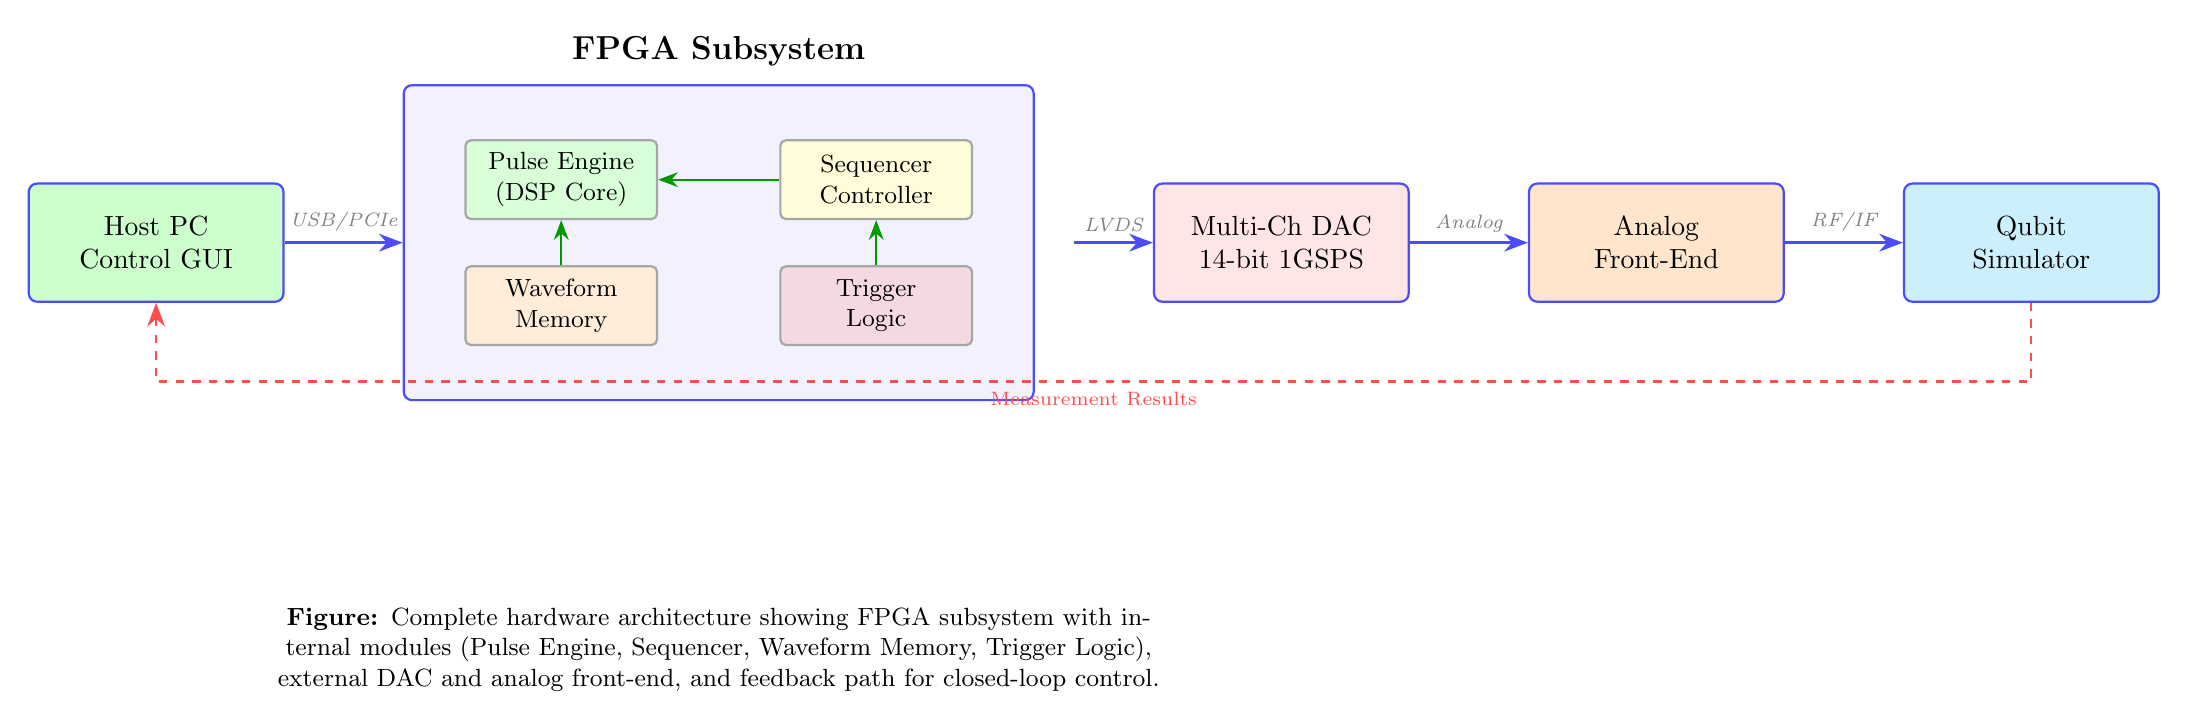
\begin{tikzpicture}[
    mainblock/.style={rectangle, draw=blue!70, fill=blue!10, thick, text width=3cm, text centered, minimum height=1.5cm, rounded corners=3pt},
    subblock/.style={rectangle, draw=gray!70, fill=gray!10, thick, text width=2.2cm, text centered, minimum height=1cm, rounded corners=2pt, font=\small},
    arrow/.style={-{Stealth[length=3mm]}, thick, blue!70},
    dataarrow/.style={-{Stealth[length=2.5mm]}, thick, green!60!black},
    label/.style={font=\scriptsize\itshape, text=gray},
    node distance=0.8cm
]
    % FPGA Block with internal components
    \node[mainblock, minimum width=8cm, minimum height=4cm, fill=blue!5] (fpga_box) {};
    \node[above=0.1cm of fpga_box.north, font=\bfseries\large] {FPGA Subsystem};
    
    % Internal FPGA blocks
    \node[subblock, fill=green!15] (pulseeng) at ([xshift=-2cm, yshift=0.8cm]fpga_box.center) {Pulse Engine\\(DSP Core)};
    \node[subblock, fill=yellow!15] (seqctrl) at ([xshift=2cm, yshift=0.8cm]fpga_box.center) {Sequencer\\Controller};
    \node[subblock, fill=orange!15] (wfmem) at ([xshift=-2cm, yshift=-0.8cm]fpga_box.center) {Waveform\\Memory};
    \node[subblock, fill=purple!15] (triglog) at ([xshift=2cm, yshift=-0.8cm]fpga_box.center) {Trigger\\Logic};
    
    % Internal connections
    \draw[dataarrow] (wfmem) -- (pulseeng);
    \draw[dataarrow] (seqctrl) -- (pulseeng);
    \draw[dataarrow] (triglog) -- (seqctrl);
    
    % External blocks
    \node[mainblock, left=1.5cm of fpga_box, fill=green!20] (host) {Host PC\\Control GUI};
    \node[mainblock, right=1.5cm of fpga_box, fill=red!10] (dac) {Multi-Ch DAC\\14-bit 1GSPS};
    \node[mainblock, right=1.5cm of dac, fill=orange!20] (afe) {Analog\\Front-End};
    \node[mainblock, right=1.5cm of afe, fill=cyan!20] (qubit) {Qubit\\Simulator};
    
    % Main flow arrows
    \draw[arrow, very thick] (host) -- node[above, label] {USB/PCIe} (fpga_box);
    \draw[arrow, very thick] ([xshift=0.5cm]fpga_box.east) -- node[above, label] {LVDS} (dac);
    \draw[arrow, very thick] (dac) -- node[above, label] {Analog} (afe);
    \draw[arrow, very thick] (afe) -- node[above, label] {RF/IF} (qubit);
    
    % Feedback path
    \draw[arrow, dashed, thick, red!70] (qubit.south) -- ++(0,-1) -| node[below, pos=0.25, font=\scriptsize] {Measurement Results} (host.south);
    
    % Bottom labels
    \node[below=2.5cm of fpga_box, text width=12cm, text centered, font=\small] {
        \textbf{Figure:} Complete hardware architecture showing FPGA subsystem with internal modules (Pulse Engine, Sequencer, Waveform Memory, Trigger Logic), external DAC and analog front-end, and feedback path for closed-loop control.
    };
    
\end{tikzpicture}
\caption{Detailed FPGA-based pulse simulator hardware architecture with internal modules.}
\label{fig:detailed_hardware}
\end{figure}

\subsection{Project Management Flow}

\begin{figure}[htbp]
\centering
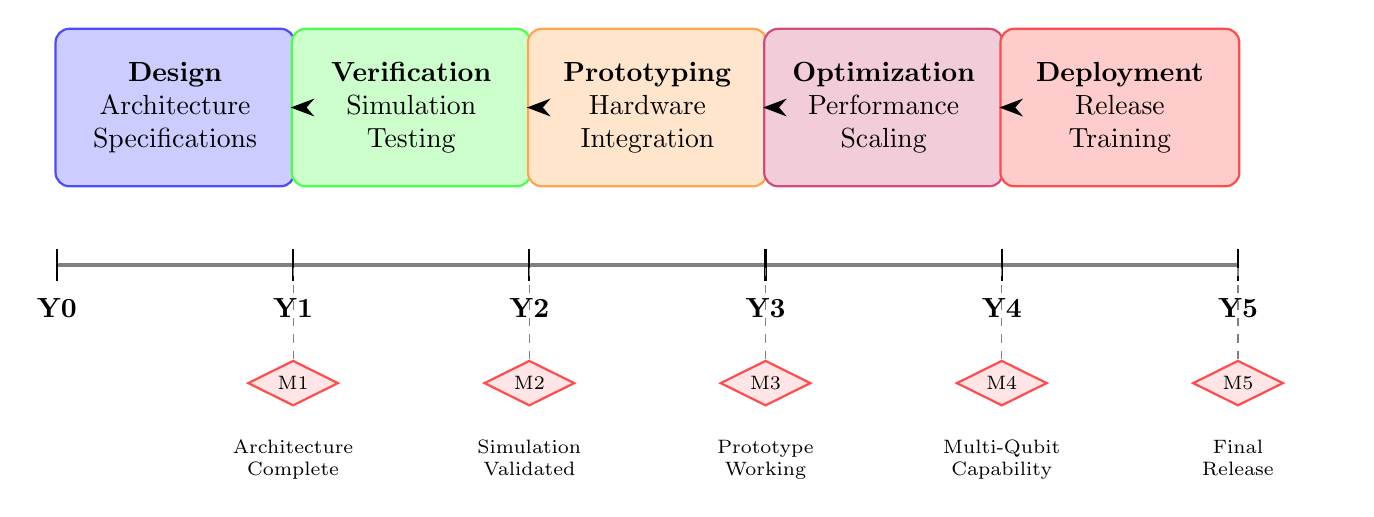
\begin{tikzpicture}[
    phase/.style={rectangle, draw=#1!70, fill=#1!20, thick, text width=2.8cm, text centered, minimum height=2cm, rounded corners=5pt},
    milestone/.style={diamond, draw=red!70, fill=red!10, thick, aspect=2, inner sep=2pt, font=\scriptsize},
    arrow/.style={-{Stealth[length=3mm]}, thick},
    timeline/.style={very thick, gray},
    node distance=0.5cm
]
    % Timeline
    \draw[timeline] (0,0) -- (15,0);
    
    % Year markers
    \foreach \x/\y in {0/Y0, 3/Y1, 6/Y2, 9/Y3, 12/Y4, 15/Y5} {
        \draw[thick] (\x,-0.2) -- (\x,0.2);
        \node[below] at (\x,-0.3) {\textbf{\y}};
    }
    
    % Phase blocks
    \node[phase=blue] (design) at (1.5,2) {\textbf{Design}\\Architecture\\Specifications};
    \node[phase=green] (verify) at (4.5,2) {\textbf{Verification}\\Simulation\\Testing};
    \node[phase=orange] (proto) at (7.5,2) {\textbf{Prototyping}\\Hardware\\Integration};
    \node[phase=purple] (optim) at (10.5,2) {\textbf{Optimization}\\Performance\\Scaling};
    \node[phase=red] (deploy) at (13.5,2) {\textbf{Deployment}\\Release\\Training};
    
    % Arrows between phases
    \draw[arrow] (design) -- (verify);
    \draw[arrow] (verify) -- (proto);
    \draw[arrow] (proto) -- (optim);
    \draw[arrow] (optim) -- (deploy);
    
    % Milestones
    \node[milestone] (m1) at (3,-1.5) {M1};
    \node[milestone] (m2) at (6,-1.5) {M2};
    \node[milestone] (m3) at (9,-1.5) {M3};
    \node[milestone] (m4) at (12,-1.5) {M4};
    \node[milestone] (m5) at (15,-1.5) {M5};
    
    % Milestone labels
    \node[below=0.3cm of m1, text width=2.5cm, text centered, font=\scriptsize] {Architecture\\Complete};
    \node[below=0.3cm of m2, text width=2.5cm, text centered, font=\scriptsize] {Simulation\\Validated};
    \node[below=0.3cm of m3, text width=2.5cm, text centered, font=\scriptsize] {Prototype\\Working};
    \node[below=0.3cm of m4, text width=2.5cm, text centered, font=\scriptsize] {Multi-Qubit\\Capability};
    \node[below=0.3cm of m5, text width=2.5cm, text centered, font=\scriptsize] {Final\\Release};
    
    % Connect milestones to timeline
    \foreach \m in {m1,m2,m3,m4,m5} {
        \draw[dashed, gray] (\m) -- (\m |- 0,0);
    }
    
\end{tikzpicture}
\caption{Project workflow showing five phases from design to deployment with major milestones.}
\label{fig:project_flow}
\end{figure}

\subsection{Software Stack Architecture}

\begin{figure}[htbp]
\centering
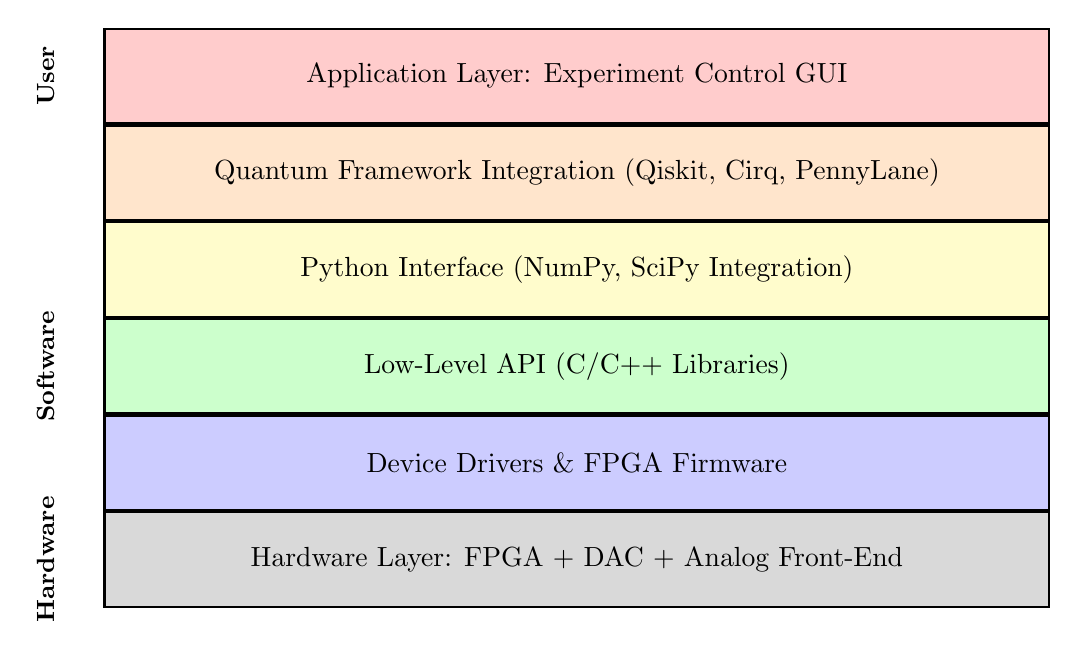
\begin{tikzpicture}[
    layer/.style={rectangle, draw=black, thick, minimum width=12cm, minimum height=1.2cm, text centered},
    node distance=0cm
]
    % Layers from bottom to top
    \node[layer, fill=gray!30] (hw) {Hardware Layer: FPGA + DAC + Analog Front-End};
    \node[layer, fill=blue!20, above=of hw] (driver) {Device Drivers \& FPGA Firmware};
    \node[layer, fill=green!20, above=of driver] (api) {Low-Level API (C/C++ Libraries)};
    \node[layer, fill=yellow!20, above=of api] (python) {Python Interface (NumPy, SciPy Integration)};
    \node[layer, fill=orange!20, above=of python] (framework) {Quantum Framework Integration (Qiskit, Cirq, PennyLane)};
    \node[layer, fill=red!20, above=of framework] (app) {Application Layer: Experiment Control GUI};
    
    % Side labels
    \node[left=0.5cm of hw, rotate=90, anchor=south, font=\small\bfseries] {Hardware};
    \node[left=0.5cm of api, rotate=90, anchor=south, font=\small\bfseries] {Software};
    \node[left=0.5cm of app, rotate=90, anchor=south, font=\small\bfseries] {User};
    
\end{tikzpicture}
\caption{Software stack architecture from hardware to application layer.}
\label{fig:software_stack}
\end{figure}

%=============================================================================
% SECTION 5: PROJECT MILESTONES
%=============================================================================
\section{Project Milestones and Quarterly Deliverables}
\label{sec:milestones}

\subsection{Five-Year Roadmap Overview}

\begin{table}[htbp]
\centering
\caption{Five-year project roadmap with key objectives}
\label{tab:roadmap}
\begin{tabular}{@{}clp{8cm}@{}}
\toprule
\textbf{Year} & \textbf{Phase} & \textbf{Key Objectives} \\
\midrule
1 & Foundation & Architecture design, FPGA prototyping, initial pulse libraries \\
2 & Development & Expanded pulse sets, Hamiltonian validation, quantum simulator integration \\
3 & Integration & Hardware-software co-design, benchmarking against classical simulators \\
4 & Optimization & Performance tuning, multi-qubit scaling, training module development \\
5 & Deployment & Final deployment, documentation, open-source release, industry workshops \\
\bottomrule
\end{tabular}
\end{table}

\subsection{Detailed Quarterly Deliverables}

\subsubsection{Year 1: Foundation Phase}

\begin{longtable}{@{}p{1.5cm}p{4cm}p{7cm}@{}}
\caption{Year 1 quarterly deliverables} \label{tab:year1} \\
\toprule
\textbf{Quarter} & \textbf{Deliverable} & \textbf{Description} \\
\midrule
\endfirsthead
\toprule
\textbf{Quarter} & \textbf{Deliverable} & \textbf{Description} \\
\midrule
\endhead
Q1 & System Requirements Document & Complete specification of performance targets, interfaces, and constraints. Review with MeitY. \\
\midrule
Q2 & Architecture Design Document & Detailed block diagrams, signal flow, FPGA resource allocation, DAC selection. \\
\midrule
Q3 & Initial FPGA Bitstream & First working FPGA implementation generating basic Gaussian pulses. Verification on evaluation board. \\
\midrule
Q4 & Basic Pulse Library (v1.0) & Implementation of 10 standard pulse shapes (Gaussian, DRAG, flat-top, etc.). Test report. \\
\bottomrule
\end{longtable}

\subsubsection{Year 2: Development Phase}

\begin{longtable}{@{}p{1.5cm}p{4cm}p{7cm}@{}}
\caption{Year 2 quarterly deliverables} \label{tab:year2} \\
\toprule
\textbf{Quarter} & \textbf{Deliverable} & \textbf{Description} \\
\midrule
\endfirsthead
Q1 & Extended Pulse Library (v2.0) & 30+ pulse shapes including composite pulses and optimized sequences. \\
\midrule
Q2 & Hamiltonian Simulator & Software module simulating qubit dynamics under generated pulses. Validation against analytical solutions. \\
\midrule
Q3 & Qiskit Integration & Backend provider for Qiskit allowing pulse-level simulation of quantum circuits. \\
\midrule
Q4 & Multi-Channel DAC Integration & Hardware integration of 8-channel DAC system. Synchronization verification. \\
\bottomrule
\end{longtable}

\subsubsection{Year 3: Integration Phase}

\begin{longtable}{@{}p{1.5cm}p{4cm}p{7cm}@{}}
\caption{Year 3 quarterly deliverables} \label{tab:year3} \\
\toprule
\textbf{Quarter} & \textbf{Deliverable} & \textbf{Description} \\
\midrule
\endfirsthead
Q1 & Integrated Prototype & Complete hardware-software system demonstration. Technical review. \\
\midrule
Q2 & Benchmark Report & Performance comparison with commercial systems and classical simulators. \\
\midrule
Q3 & Cirq/PennyLane Integration & Support for additional quantum computing frameworks. \\
\midrule
Q4 & GUI Application (v1.0) & User-friendly graphical interface for experiment control and visualization. \\
\bottomrule
\end{longtable}

\subsubsection{Year 4: Optimization Phase}

\begin{longtable}{@{}p{1.5cm}p{4cm}p{7cm}@{}}
\caption{Year 4 quarterly deliverables} \label{tab:year4} \\
\toprule
\textbf{Quarter} & \textbf{Deliverable} & \textbf{Description} \\
\midrule
\endfirsthead
Q1 & Performance Optimization & Timing jitter reduction to $<0.5$ ns. Amplitude accuracy improvement. \\
\midrule
Q2 & Multi-Qubit Extension & Scaling to 16-qubit pulse simulation capability. Crosstalk mitigation. \\
\midrule
Q3 & Training Module (Draft) & Course materials for FPGA design and quantum control. \\
\midrule
Q4 & Pilot Training Program & First training batch of 20 engineers from academic institutions. \\
\bottomrule
\end{longtable}

\subsubsection{Year 5: Deployment Phase}

\begin{longtable}{@{}p{1.5cm}p{4cm}p{7cm}@{}}
\caption{Year 5 quarterly deliverables} \label{tab:year5} \\
\toprule
\textbf{Quarter} & \textbf{Deliverable} & \textbf{Description} \\
\midrule
\endfirsthead
Q1 & Production Version & Final hardware and software release candidate. \\
\midrule
Q2 & Documentation Suite & Complete user manual, API documentation, and application notes. \\
\midrule
Q3 & Open-Source Release & Public release of software components on GitHub. Community setup. \\
\midrule
Q4 & Industry Workshops & Three workshops at major institutions. Technology transfer completion. \\
\bottomrule
\end{longtable}

\subsection{Milestone Summary Chart}

\begin{figure}[htbp]
\centering
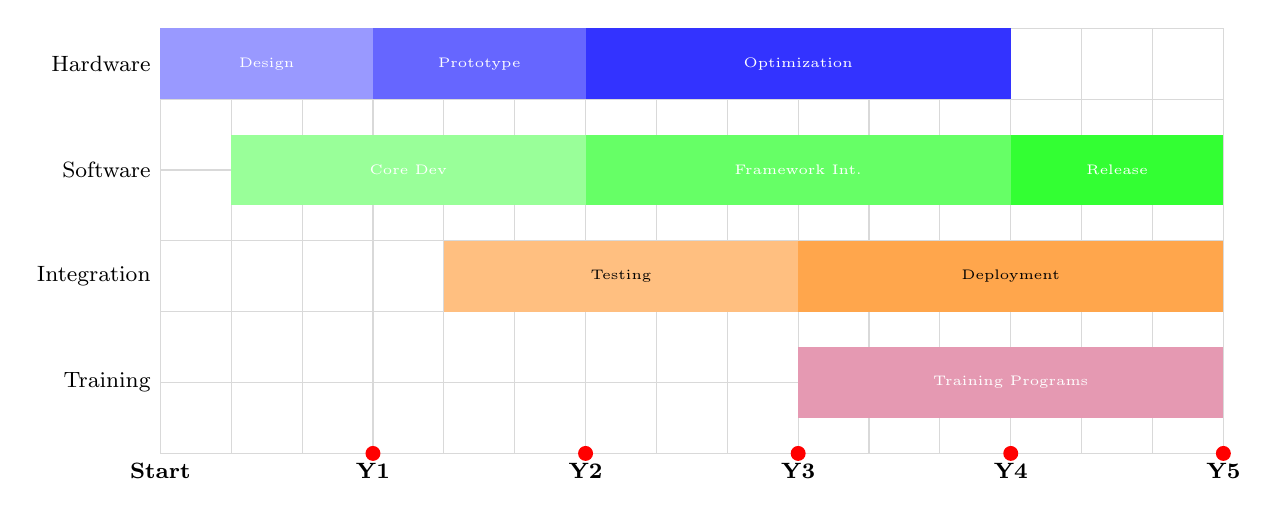
\begin{tikzpicture}[scale=0.9]
    % Grid
    \draw[gray!30] (0,0) grid (15,6);
    
    % Year labels
    \foreach \x/\y in {0/Start, 3/Y1, 6/Y2, 9/Y3, 12/Y4, 15/Y5} {
        \node[below, font=\footnotesize\bfseries] at (\x,0) {\y};
    }
    
    % Category labels
    \node[left, font=\footnotesize] at (0,5.5) {Hardware};
    \node[left, font=\footnotesize] at (0,4) {Software};
    \node[left, font=\footnotesize] at (0,2.5) {Integration};
    \node[left, font=\footnotesize] at (0,1) {Training};
    
    % Hardware timeline
    \fill[blue!40] (0,5) rectangle (3,6);
    \fill[blue!60] (3,5) rectangle (6,6);
    \fill[blue!80] (6,5) rectangle (12,6);
    \node[font=\tiny, white] at (1.5,5.5) {Design};
    \node[font=\tiny, white] at (4.5,5.5) {Prototype};
    \node[font=\tiny, white] at (9,5.5) {Optimization};
    
    % Software timeline
    \fill[green!40] (1,3.5) rectangle (6,4.5);
    \fill[green!60] (6,3.5) rectangle (12,4.5);
    \fill[green!80] (12,3.5) rectangle (15,4.5);
    \node[font=\tiny, white] at (3.5,4) {Core Dev};
    \node[font=\tiny, white] at (9,4) {Framework Int.};
    \node[font=\tiny, white] at (13.5,4) {Release};
    
    % Integration timeline
    \fill[orange!50] (4,2) rectangle (9,3);
    \fill[orange!70] (9,2) rectangle (15,3);
    \node[font=\tiny] at (6.5,2.5) {Testing};
    \node[font=\tiny] at (12,2.5) {Deployment};
    
    % Training timeline
    \fill[purple!40] (9,0.5) rectangle (15,1.5);
    \node[font=\tiny, white] at (12,1) {Training Programs};
    
    % Milestones
    \foreach \x in {3,6,9,12,15} {
        \fill[red] (\x,0) circle (3pt);
    }
    
\end{tikzpicture}
\caption{Gantt-style overview of project phases across five years.}
\label{fig:gantt}
\end{figure}

%=============================================================================
% SECTION 6: COST STRUCTURE
%=============================================================================
\section{Cost Structure}
\label{sec:cost}

\subsection{Budget Summary}

The total project budget is \crore{5.0} distributed as follows:

\begin{table}[htbp]
\centering
\caption{Budget allocation summary}
\label{tab:budget}
\begin{tabular}{@{}lrrr@{}}
\toprule
\textbf{Category} & \textbf{Amount (\crore{})} & \textbf{Percentage} & \textbf{Per Year (Avg)} \\
\midrule
Hardware Procurement & 2.00 & 40\% & 0.40 \\
Manpower & 1.50 & 30\% & 0.30 \\
Software Tools/Licenses & 0.50 & 10\% & 0.10 \\
Training \& Dissemination & 0.50 & 10\% & 0.10 \\
Contingency \& Overheads & 0.50 & 10\% & 0.10 \\
\midrule
\textbf{Total} & \textbf{5.00} & \textbf{100\%} & \textbf{1.00} \\
\bottomrule
\end{tabular}
\end{table}

\subsection{Detailed Cost Breakdown}

\subsubsection{Hardware Procurement (\crore{2.0})}

\begin{table}[htbp]
\centering
\caption{Hardware procurement details}
\label{tab:hardware_cost}
\begin{tabular}{@{}p{5cm}rrr@{}}
\toprule
\textbf{Item} & \textbf{Qty} & \textbf{Unit Cost (₹ Lakhs)} & \textbf{Total (₹ Lakhs)} \\
\midrule
Xilinx Ultrascale+ FPGA Dev Kits & 5 & 15.0 & 75.0 \\
High-Speed DAC Modules (1 GSPS) & 10 & 8.0 & 80.0 \\
RF Signal Generators & 4 & 5.0 & 20.0 \\
Oscilloscopes (High BW) & 3 & 8.0 & 24.0 \\
Spectrum Analyzers & 2 & 6.0 & 12.0 \\
Workstations \& Servers & 8 & 3.0 & 24.0 \\
Networking \& Infrastructure & 1 & 10.0 & 10.0 \\
Miscellaneous Components & -- & -- & 55.0 \\
\midrule
\textbf{Subtotal} & & & \textbf{200.0} \\
\bottomrule
\end{tabular}
\end{table}

\subsubsection{Manpower (\crore{1.5})}

\begin{table}[htbp]
\centering
\caption{Manpower allocation over 5 years}
\label{tab:manpower_cost}
\begin{tabular}{@{}p{4cm}rrrr@{}}
\toprule
\textbf{Role} & \textbf{Count} & \textbf{Monthly (₹ Lakhs)} & \textbf{Duration (Months)} & \textbf{Total (₹ Lakhs)} \\
\midrule
Project Lead (Senior Scientist) & 1 & 1.5 & 60 & 90.0 \\
FPGA Engineers & 3 & 0.8 & 60 & 144.0 \\
Software Developers & 2 & 0.7 & 48 & 67.2 \\
Research Associates & 2 & 0.5 & 36 & 36.0 \\
Project Coordinator & 1 & 0.4 & 60 & 24.0 \\
\midrule
\textbf{Subtotal} & & & & \textbf{150.0} \\
\bottomrule
\end{tabular}
\end{table}

\subsubsection{Software Tools and Licenses (\crore{0.5})}

\begin{table}[htbp]
\centering
\caption{Software and license costs}
\label{tab:software_cost}
\begin{tabular}{@{}p{6cm}rr@{}}
\toprule
\textbf{Software/Tool} & \textbf{Annual (₹ Lakhs)} & \textbf{5-Year Total (₹ Lakhs)} \\
\midrule
Xilinx Vivado Design Suite (Enterprise) & 5.0 & 25.0 \\
MATLAB/Simulink (with HDL Coder) & 3.0 & 15.0 \\
CAD Tools (PCB Design) & 1.0 & 5.0 \\
Cloud Computing Resources & 1.0 & 5.0 \\
\midrule
\textbf{Subtotal} & & \textbf{50.0} \\
\bottomrule
\end{tabular}
\end{table}

\subsubsection{Training, Workshops, and Dissemination (\crore{0.5})}

\begin{itemize}
    \item \textbf{Workshop Organization:} ₹20 Lakhs (5 workshops × ₹4 Lakhs each)
    \item \textbf{Conference Participation:} ₹10 Lakhs (international conferences, publications)
    \item \textbf{Training Material Development:} ₹10 Lakhs
    \item \textbf{Outreach and Documentation:} ₹10 Lakhs
\end{itemize}

\subsubsection{Contingency and Overheads (\crore{0.5})}

\begin{itemize}
    \item \textbf{Equipment Maintenance:} ₹15 Lakhs
    \item \textbf{Travel and Coordination:} ₹10 Lakhs
    \item \textbf{Institutional Overheads:} ₹15 Lakhs
    \item \textbf{Contingency Reserve:} ₹10 Lakhs
\end{itemize}

\subsection{Year-wise Expenditure Plan}

\begin{table}[htbp]
\centering
\caption{Year-wise budget distribution (₹ Lakhs)}
\label{tab:yearly_budget}
\begin{tabular}{@{}lrrrrr|r@{}}
\toprule
\textbf{Category} & \textbf{Y1} & \textbf{Y2} & \textbf{Y3} & \textbf{Y4} & \textbf{Y5} & \textbf{Total} \\
\midrule
Hardware & 80 & 50 & 30 & 25 & 15 & 200 \\
Manpower & 25 & 30 & 32 & 33 & 30 & 150 \\
Software & 12 & 10 & 10 & 10 & 8 & 50 \\
Training & 5 & 8 & 10 & 12 & 15 & 50 \\
Contingency & 8 & 10 & 10 & 12 & 10 & 50 \\
\midrule
\textbf{Total} & \textbf{130} & \textbf{108} & \textbf{92} & \textbf{92} & \textbf{78} & \textbf{500} \\
\bottomrule
\end{tabular}
\end{table}

\subsection{Budget Visualization}

\begin{figure}[htbp]
\centering
\begin{tikzpicture}
\pie[
    text=legend,
    radius=3,
    color={blue!60, green!60, orange!60, purple!60, gray!60}
]{
    40/Hardware (₹2.0 Cr),
    30/Manpower (₹1.5 Cr),
    10/Software (₹0.5 Cr),
    10/Training (₹0.5 Cr),
    10/Contingency (₹0.5 Cr)
}
\end{tikzpicture}
\caption{Budget distribution across major categories.}
\label{fig:budget_pie}
\end{figure}

%=============================================================================
% SECTION 7: ACHIEVABILITY AND RISK MITIGATION
%=============================================================================
\section{Achievability and Risk Mitigation}
\label{sec:risk}

\subsection{CDAC's Prior Expertise}

CDAC Noida brings substantial expertise to this project:

\begin{itemize}
    \item \textbf{FPGA Development:} Over 20 years of experience in FPGA-based system design for defense, telecommunications, and scientific applications.
    
    \item \textbf{High-Speed Digital Design:} Successfully delivered multi-gigahertz digital systems for ISRO and DRDO.
    
    \item \textbf{Signal Processing:} Extensive experience in digital signal processing for radar, communication, and instrumentation.
    
    \item \textbf{Supercomputing:} PARAM series development demonstrates capability in complex system integration.
    
    \item \textbf{Quantum Computing Interest:} Active participation in National Quantum Mission planning and quantum software development.
\end{itemize}

\subsection{Achievability Assessment}

\begin{table}[htbp]
\centering
\caption{Technical achievability assessment}
\label{tab:achievability}
\begin{tabular}{@{}p{4cm}p{2cm}p{6cm}@{}}
\toprule
\textbf{Objective} & \textbf{Risk Level} & \textbf{Justification} \\
\midrule
FPGA pulse generation & Low & Well-established technique; commercial examples exist \\
Sub-ns timing resolution & Medium & Requires careful design but achievable with modern FPGAs \\
Multi-channel DAC integration & Low & Standard engineering task; components available \\
Quantum framework integration & Medium & Requires software expertise; APIs well-documented \\
Multi-qubit scaling & Medium-High & Complex but modular approach reduces risk \\
Training program delivery & Low & CDAC has established training infrastructure \\
\bottomrule
\end{tabular}
\end{table}

\subsection{Risk Identification and Mitigation}

\begin{table}[htbp]
\centering
\caption{Risk register with mitigation strategies}
\label{tab:risks}
\begin{tabular}{@{}p{3cm}p{1.5cm}p{1.5cm}p{6cm}@{}}
\toprule
\textbf{Risk} & \textbf{Likelihood} & \textbf{Impact} & \textbf{Mitigation Strategy} \\
\midrule
FPGA component shortage & Medium & High & Maintain inventory buffer; identify alternative suppliers; design for multiple FPGA families \\
\midrule
Performance targets not met & Medium & Medium & Iterative design approach; early prototyping; fallback to reduced specifications \\
\midrule
Integration challenges & Medium & Medium & Modular architecture; extensive testing at each stage; parallel development tracks \\
\midrule
Key personnel departure & Low & High & Knowledge documentation; cross-training; competitive compensation \\
\midrule
Technology obsolescence & Low & Medium & Design for upgradeability; abstract hardware interfaces; monitor industry trends \\
\midrule
Budget overrun & Low & Medium & Quarterly reviews; contingency reserve; phased procurement \\
\bottomrule
\end{tabular}
\end{table}

\subsection{Fallback Strategies}

\subsubsection{Classical Simulator Fallback}
If hardware development faces significant delays, the software Hamiltonian simulator can operate independently on classical computers, providing immediate value to researchers while hardware issues are resolved.

\subsubsection{Modular FPGA Design}
The modular architecture allows:
\begin{itemize}
    \item Individual modules to be upgraded independently
    \item Partial functionality delivery even if some components face delays
    \item Easy adaptation to different FPGA platforms if supply issues arise
\end{itemize}

\subsubsection{Reduced Scope Option}
If necessary, the project can deliver a fully functional 4-channel system instead of 16-channel, still providing significant research capability.

\subsection{Quality Assurance}

\begin{enumerate}
    \item \textbf{Quarterly Reviews:} Progress assessment with MeitY representatives
    \item \textbf{External Advisory Board:} Annual review by domain experts from IITs and research institutions
    \item \textbf{Documentation Standards:} IEEE documentation standards for all technical deliverables
    \item \textbf{Testing Protocol:} Comprehensive verification and validation at each milestone
\end{enumerate}

%=============================================================================
% SECTION 8: CONCLUSION
%=============================================================================
\section{Conclusion}
\label{sec:conclusion}

\subsection{Summary of Proposal}

This proposal presents a compelling case for MeitY funding of the \textbf{FPGA-Based Pulse Simulator for Quantum and Classical Signal Research} project. The key points are:

\begin{enumerate}
    \item \textbf{Strategic Importance:} The project directly supports India's National Quantum Mission by creating indigenous capabilities in quantum control hardware.
    
    \item \textbf{Technical Feasibility:} Building on CDAC's proven expertise in FPGA systems, the project follows a well-defined technical roadmap with manageable risks.
    
    \item \textbf{Clear Deliverables:} Twenty quarterly milestones over five years ensure measurable progress and accountability.
    
    \item \textbf{Contained Costs:} The \crore{5.0} budget is competitive compared to importing equivalent capabilities.
    
    \item \textbf{Lasting Impact:} Open-source release and trained workforce create sustainable benefits beyond the project duration.
\end{enumerate}

\subsection{National Impact}

The successful completion of this project will:

\begin{itemize}
    \item Enable Indian researchers to develop and test quantum algorithms without dependence on foreign hardware
    \item Create a cadre of engineers skilled in quantum control techniques
    \item Establish CDAC as a center of excellence in quantum hardware infrastructure
    \item Contribute to India's self-reliance in strategic technologies
    \item Foster industry-academia collaboration in quantum technology
\end{itemize}

\subsection{Call to Action}

We respectfully request MeitY to approve funding for this project. The investment will yield:

\begin{itemize}
    \item Tangible hardware and software deliverables
    \item Skilled human resources for India's quantum future
    \item Research publications enhancing India's global standing
    \item Open-source contributions benefiting the worldwide community
    \item Strategic autonomy in a critical technology domain
\end{itemize}

\begin{center}
\fbox{
\parbox{0.8\textwidth}{
\centering
\textbf{The FPGA-Based Pulse Simulator project represents a strategic investment in India's quantum future. With clear objectives, proven capabilities, and contained costs, it offers exceptional value for MeitY's mission of advancing India's electronics and IT ecosystem.}
}
}
\end{center}

%=============================================================================
% SECTION 9: REFERENCES
%=============================================================================
\newpage
\printbibliography[heading=bibintoc, title={References}]

%=============================================================================
% APPENDICES
%=============================================================================
\appendix

\section{Abbreviations}
\label{app:abbreviations}

\begin{table}[htbp]
\centering
\begin{tabular}{@{}ll@{}}
\toprule
\textbf{Abbreviation} & \textbf{Full Form} \\
\midrule
CDAC & Centre for Development of Advanced Computing \\
DAC & Digital-to-Analog Converter \\
DRAG & Derivative Removal by Adiabatic Gate \\
DSP & Digital Signal Processing \\
FPGA & Field-Programmable Gate Array \\
GSPS & Giga Samples Per Second \\
GUI & Graphical User Interface \\
MeitY & Ministry of Electronics and Information Technology \\
RF & Radio Frequency \\
\bottomrule
\end{tabular}
\end{table}

\section{Team Composition}
\label{app:team}

\begin{table}[htbp]
\centering
\begin{tabular}{@{}p{3cm}p{4cm}p{5cm}@{}}
\toprule
\textbf{Role} & \textbf{Qualifications} & \textbf{Responsibilities} \\
\midrule
Project Lead & Ph.D. in Electronics/Physics, 15+ years experience & Overall technical direction, MeitY liaison \\
FPGA Engineers & M.Tech in VLSI/Embedded, 5+ years experience & Hardware design, firmware development \\
Software Developers & M.Tech in CS, 3+ years experience & API development, framework integration \\
Research Associates & M.Sc./M.Tech, 0-3 years experience & Testing, documentation, research support \\
Project Coordinator & MBA/M.Tech, 5+ years PM experience & Schedule, budget, reporting \\
\bottomrule
\end{tabular}
\end{table}

\end{document}
